\documentclass[review,authoryear,3p,times]{elsarticle}
% EJOR submission. 3p = 3-part (author) layout; `review` for double spacing;
% `authoryear` for (Author, year) citations via elsarticle-harv.
% v2 draft (2026-08-03): full rewrite around the two-mechanism + boundary-
% condition structure (see ../EJOR_PAPER_OUTLINE.md). Does not reuse v1's
% narrative spine section-by-section; the Background/Method-4a/Theory-P1-P2
% content is carried over near-verbatim where the underlying result is
% unchanged (s-ccf), everything else is new.

\usepackage{amsmath,amssymb,amsthm}
\usepackage{graphicx}
\usepackage{booktabs}
\usepackage{algorithm}
\usepackage{algpseudocode}
\usepackage{tikz}
\usetikzlibrary{petri,positioning,arrows.meta,fit,backgrounds,calc}
\usepackage[hidelinks]{hyperref}

\newtheorem{proposition}{Proposition}
\newtheorem{corollary}{Corollary}
\newtheorem{assumption}{Assumption}
\newtheorem{remark}{Remark}

\newcommand{\ccf}{\textsc{ccf}}
\newcommand{\sccf}{\textsc{s-ccf}}
\newcommand{\mcq}{\textsc{mc-q}}
\newcommand{\lrq}{\textsc{lrq}}
\newcommand{\cfpk}{\textsc{cfpk}}
\newcommand{\Kstat}{K_{\mathrm{stat}}}
\newcommand{\Krea}{K_{\mathrm{real}}}
\newcommand{\Fscr}{\mathcal{F}}
\newcommand{\Ascr}{\mathcal{A}}
\newcommand{\Ex}{\mathbb{E}}
\newcommand{\Var}{\operatorname{Var}}
\newcommand{\Cov}{\operatorname{Cov}}

\journal{European Journal of Operational Research}

\begin{document}

\begin{frontmatter}

\title{Exploiting Causal Provenance for Credit Assignment in Reinforcement
Learning for Dynamic Task Assignment: Mechanisms, Guarantees, and Limits}

\author[tue]{Riccardo Lo Bianco\corref{cor}}
\ead{r.lo.bianco@tue.nl}
\cortext[cor]{Corresponding author.}
\author[tue]{Co-authors \textnormal{(TODO)}}
\address[tue]{Eindhoven University of Technology, Eindhoven, The Netherlands}

\begin{abstract}
Dynamic task assignment problems---allocating stochastic streams of tasks to
limited, contended resources---are increasingly solved by deep reinforcement
learning (DRL) over executable process models such as Action-Evolution Petri
Nets (A-E PN). Existing approaches treat the model as a black-box (semi-)Markov
decision process and apply generic policy-gradient methods (PPO), discarding the
\emph{causal provenance} the Petri net records for free: which past decisions
influenced which rewards. We show this provenance can be exploited for credit
assignment in two complementary ways. First, \sccf{} partitions each episode's
decisions into causal components by union-find over reward provenance and
credits every decision only with its own component's discounted reward-to-go;
we prove it is an unbiased, variance-reducing policy-gradient estimator, show
that its naive realized-partition predecessor (\ccf) is in fact biased at
shared-resource handoffs (an exact sign-flip demonstration), and that the fix
requires only computing the partition from the static net topology instead.
Second, \cfpk{} uses provenance not as a filter but as a replayable causal
model: it forks the simulator to obtain an \emph{exact} per-decision
counterfactual credit, and we prove a novel cost reduction---coupling
truncation---that shares one simulated continuation between the two forked
branches whenever they provably reconverge, which we show cancels exactly in
the estimator (not merely reduces variance) and measure a $1.37\times$
wall-clock speedup with byte-identical training outcomes. Empirically, \sccf{}
reduces to PPO when the system forms a single causal component (a
shared-bottleneck queue), correctly tying it, and beats PPO decisively as
concurrent independence grows, including on a realistic multi-site
skills-based routing problem where PPO fails to learn (normalized return
$0.15$) while \sccf{} succeeds ($0.52$, $p=0.005$, Cohen's $d=1.27$), at
essentially the same computational cost. Finally, we investigate whether the
honest null both mechanisms predict on a genuinely single-component
bottleneck can be closed by any other provenance- or structure-exploiting
route, and rule out three independently-motivated candidates with proofs
rather than single discouraging runs: potential-based reward shaping (safe by
theorem, empirically counter-productive at practical budgets), static
structural input features (provably redundant given the network's existing
action-type encoding), and a previously undocumented graph-actor
architecture blind spot, which we prove is real via exact-invariance under
an untrained network, fix, and show still does not move the bottleneck. This
precisely localizes the bottleneck's remaining difficulty away from credit
assignment and observability---a decision rule for practitioners as much as
a technical result.
\end{abstract}

\begin{keyword}
Reinforcement learning \sep Credit assignment \sep Dynamic task assignment \sep
Petri nets \sep Decomposition \sep Counterfactual reasoning \sep Variance
reduction \sep Graph neural networks
\end{keyword}

\end{frontmatter}

% ======================================================================
\section{Introduction}
\label{sec:intro}

Dynamic task assignment is a core operational problem: a stream of tasks arrives
stochastically and must be allocated, over time, to a limited set of contended
resources so as to optimize a throughput or cost objective. It underlies
scheduling, service-system staffing, manufacturing control, and business-process
operation. A recent line of work models such problems with \emph{Action-Evolution
Petri Nets} (A-E PN), an executable formalism that unifies Markov decision
processes with colored Petri nets, and solves them with deep reinforcement
learning \citep{aepn2023,aepn_repr2025,gympn2025}. This program has established
that A-E PN can \emph{model} a broad taxonomy of assignment problems, that a
graph-based representation makes them learnable at scale, and that a software
library makes the whole pipeline practical.

In every case, however, the \emph{learning engine} is a generic policy-gradient
method---typically Proximal Policy Optimization (PPO) \citep{ppo2017}---applied
to the induced (semi-)Markov decision process as if it were a black box. This
discards structure that the Petri net makes explicit and records for free: the
\emph{token provenance}, i.e.\ which tokens were consumed and produced by each
transition firing, and hence which past decisions lie on the causal lineage of
each reward.

\paragraph{The problem.} Policy-gradient methods credit each decision with the
\emph{return-to-go}: the sum of all rewards occurring after it, minus a learned
baseline. In a system where many cases flow concurrently, the return-to-go of a
decision about case~$i$ includes the rewards of every other case that happens to
complete afterwards---rewards the decision had no causal influence over. The
critic removes the \emph{mean} of this cross-case reward, but not its
\emph{variance}. With $K$ independent cases in flight, a single decision's
advantage carries the reward variance of all $K$, so the learning signal is
buried in concurrent-case noise, and the noise grows with concurrency. This is
the multi-entity credit-assignment problem that difference rewards
\citep{difference2002} and value decomposition \citep{coma2018,vdn2018,qmix2018}
were designed for---but those methods require the entity partition to be
specified by hand.

\paragraph{Our approach.} We exploit token provenance to solve this in two
complementary ways, spanning a bias/variance/granularity/cost spectrum, and we
report a third, equally rigorous investigation into where this kind of
exploitation stops paying off. First, for each episode we build the lineage
DAG and, for each reward, union the decisions on its causal ancestry into a
single \emph{causal component}; each decision is then credited only with its
own component's discounted reward-to-go (\sccf). In OR terms this is a
\emph{decomposition} method---in the lineage of Benders and Dantzig--Wolfe, we
decompose the policy-gradient return along the causal-component structure of
the stochastic system---but the decomposition is discovered per episode from
provenance rather than imposed a priori. Second, rather than partition
anything, \cfpk{} forks the simulator at a decision and replays the true
environment dynamics under the taken action and an alternative from the
identical pre-decision state, obtaining an \emph{exact} counterfactual credit
with no partition to get wrong; we show its dominant extra cost can be
reduced, exactly and for free, whenever the two forked branches provably
reconverge to a common state. Third, having established precisely when these
mechanisms help---and, by the same theory, precisely when they collapse to a
no-op---we ask whether the residual gap on a single-component bottleneck can
be closed by any other route that only changes what the learner observes, and
show, with proofs rather than speculation, that three well-motivated
candidates cannot.

\paragraph{Contributions.}
\begin{enumerate}
\item We identify that generic policy-gradient RL discards the provenance
structure A-E PN makes explicit, and that this causes credit-assignment
variance that grows with concurrent independence (Section~\ref{sec:method}).
\item \textbf{\sccf}: a structure-\emph{derived} (not hand-specified) factored
credit method, computed by union-find over the \emph{static} net topology.
We prove it is unbiased and variance-reducing (Propositions~\ref{prop:unbiased}--
\ref{prop:var}, Corollary~\ref{cor:mono}), and give an exact sign-flip
demonstration that its naive realized-partition predecessor \ccf{} is biased
at shared-resource handoffs, which \sccf{} fixes by construction
(Proposition~\ref{prop:sccf}; Sections~\ref{sec:method},~\ref{sec:theory},~\ref{sec:experiments}).
\item \textbf{\cfpk}: provenance used as a replayable causal model for
\emph{exact} counterfactual credit, with a novel, provably lossless cost
reduction (coupling truncation, Proposition~\ref{prop:coupling}) measured at
a $1.37\times$ wall-clock speedup with byte-identical training outcomes
(Sections~\ref{sec:method},~\ref{sec:theory},~\ref{sec:experiments}).
\item Empirically, \sccf{} reduces exactly to PPO on single-component
problems and beats it decisively as independence grows, including on a
realistic multi-site skills-based routing problem, at $\sim\!1\times$ the
compute (Section~\ref{sec:experiments}).
\item A rigorous characterization of the \emph{boundary} of provenance
exploitation: we stress-test three independent, well-motivated alternative
routes to closing the honest null both mechanisms predict on a
single-component bottleneck---denser reward signal, richer structural input
features, and a more observant graph-actor architecture---and show each is
either provably inert or empirically neutral, via proofs and exact-invariance
tests rather than single discouraging runs (Section~\ref{sec:boundary}). This
localizes the bottleneck's remaining difficulty away from credit assignment
and observability, giving practitioners a decision rule (Section~\ref{sec:discussion})
rather than an unconditional claim.
\end{enumerate}

% ======================================================================
\section{Related work}
\label{sec:related}

\paragraph{DRL for dynamic task assignment and operational control.} A growing
literature applies DRL to scheduling, routing, and business-process
decision-making, typically encoding the problem instance as a graph consumed
by a graph neural network policy: greedy graph-embedding heuristics for
combinatorial construction \citep{khalil2017learning}, attention-based
routing policies \citep{nazari2018vrp}, and GNN-based dispatching for job-shop
scheduling \citep{zhang2020jobshop}, the last especially close in spirit to
our setting. \citet{mazyavkina2021survey} survey this broader RL-for-
combinatorial-optimization literature; \citet{bengio2021tour}, published in
this journal, give the methodological tour d'horizon our OR framing draws on
most directly. Within the A-E PN program, \citet{aepn2023} introduce the
formalism and a taxonomy of assignment archetypes, \citet{aepn_repr2025} give
a graph representation for infinite state/action spaces, and \citet{gympn2025}
provide a library supporting partial observability and multiple decisions.
Across this literature, the learning algorithm is almost universally a black
box on top of the graph encoding; the simulator's own execution trace---which
decisions caused which outcomes---is not itself treated as a source of
learning signal. Our contribution is orthogonal to and compatible with all of
the above: it is a credit-assignment mechanism, not a new policy architecture
or problem encoding.

\paragraph{Credit assignment in RL.} Return decomposition \citep{rudder2019}
learns to redistribute return along a trajectory via a return-predicting
model's contribution analysis; Hindsight Credit Assignment \citep{hca2019}
reweights past actions by their learned likelihood of having caused an
observed outcome. Both are \emph{learned} redistribution mechanisms trained
on correlational patterns across trajectories. Our mechanisms differ in
kind: token provenance in an A-E PN is not inferred, it is recorded exactly by
the simulator, so \sccf{} and \cfpk{}'s credit signals carry no approximation
error from the attribution step itself. This is close in motivation to
model-free counterfactual credit assignment \citep{ccadeep2021}, which
conditions value functions on future events to build low-variance
counterfactual baselines; \cfpk{}'s simulator replay can be read as the model-based
analogue of the same goal, made exact because the simulator is itself an
available, cheap-to-fork causal model, not something that needs to be learned.

\paragraph{Factored / multi-agent credit.} Difference rewards
\citep{difference2002} credit each agent with its marginal contribution
relative to a counterfactual baseline; COMA \citep{coma2018} learns this
baseline via a centralized critic; value decomposition
\citep{vdn2018,qmix2018} factors a joint value across agents under additivity
or monotonicity constraints. All require the entity/agent partition to be
given. \sccf{} needs no such specification: the causal-component partition is
derived automatically, per episode, from token provenance, and can vary in
shape as the realized case mix changes---a single-agent problem (one policy,
many concurrent cases) is factored the same way a genuinely multi-agent one
would be.

\paragraph{Potential-based reward shaping.} \citet{ng1999shaping} prove that
adding a potential-based term to every step's reward cannot change an MDP's
optimal policy, for any potential function. We use the SMDP-discounted
generalization of this theorem not as a headline mechanism but as one of
three falsified alternative routes in our boundary-condition investigation
(Section~\ref{sec:boundary}): a theorem-safe, empirically counter-productive
result at practical training budgets, included because it isolates
sample-efficiency effects cleanly from the bias effects that are our main
concern in Section~\ref{sec:theory}.

\paragraph{Graph neural networks for combinatorial optimization and
heterogeneous actor-critic architectures.} GNNs are now a standard state
encoder for RL over combinatorial structures with variable size and topology
\citep{khalil2017learning,zhang2020jobshop}; our environments use a
heterogeneous variant, the Heterogeneous Graph Transformer
\citep{hu2020hgt}, encoding places and transitions as distinct node types.
Section~\ref{sec:boundary} documents an architectural finding of independent
interest: a per-node actor decoder combined with directed-only (non-reversed)
message-passing edges can be \emph{exactly} blind to state outside its
forward-reachable neighborhood, a limitation the critic (which pools) does
not share. To our knowledge this is not previously documented for
heterogeneous actor-critic graph architectures, and the argument is
orthogonal to the specific choice of GNN backbone.

\paragraph{Decomposition in operations research.} Dantzig--Wolfe decomposition
\citep{dantzig1960decomposition} and Benders decomposition
\citep{benders1962partitioning} break a hard, structured optimization problem
into a master problem and weakly-coupled subproblems along a hand-identified
block structure. \sccf{} applies the same idea to the policy-gradient
\emph{return}: decompose it along a block structure derived automatically,
per episode, from the simulator's own causal record, rather than a static
constraint matrix's block structure identified a priori.

% ======================================================================
\section{Background}
\label{sec:background}

Because Action-Evolution Petri Nets are not yet widely known, we describe the
formalism intuitively before defining the learning problem.

\paragraph{Petri nets and colored tokens.} A Petri net is a bipartite directed
graph of \emph{places} (drawn as circles) and \emph{transitions} (drawn as bars),
connected by arcs. Places hold \emph{tokens}; in a \emph{colored} net each token
carries typed data---a task's type, a resource's identity. A transition is
\emph{enabled} when its input places jointly hold a matching combination of
tokens, called a \emph{binding}; \emph{firing} the transition consumes that
binding and produces new tokens in its output places. The distribution of tokens
over places---the \emph{marking}---is the system state, and it evolves as
transitions fire.

\paragraph{The action/evolution split.} An Action-Evolution Petri Net (A-E PN)
\citep{aepn2023} partitions the transitions into two kinds and adds a global
clock. \emph{Evolution} transitions model the exogenous dynamics: they fire
automatically according to stochastic, timed rules---task arrivals, service
completions---advancing the clock. \emph{Action} transitions model the
controllable decisions: whenever several action bindings are simultaneously
enabled, an external \emph{policy} selects which one to fire. Selected firings may
carry a scalar \emph{reward}. Figure~\ref{fig:aepn} shows a minimal assignment
net: a waiting task and a free resource are consumed by an \emph{assign} action
transition---the decision of which task to serve with which resource---producing
a \emph{busy} token; an evolution transition \emph{complete} later frees the
resource (returning it to the pool) and emits a reward.

\paragraph{The induced SMDP.} Executing an A-E PN therefore alternates between the
environment evolving the marking (evolution firings that advance the clock) and
the agent choosing among enabled action bindings---exactly a semi-Markov decision
process (SMDP). We write $s_d$ for the marking at decision $d$, $a_d$ for the
chosen binding, and $u_d$ for its clock; delayed rewards are discounted by the
SMDP factor $\rho_d(t)=e^{-\beta\max(0,\,t-u_d)}$. Dynamic task assignment
problems---matching stochastic task streams to contended resources---map onto
this template directly \citep{aepn2023,aepn_repr2025,gympn2025}. Because the
simulator is a deterministic function of the marking, the clock, and the
(recorded) exogenous random draws, it can be \emph{snapshotted and re-run}
from any decision point under an alternative action---the capability
\cfpk{}'s forking (Section~\ref{sec:method}) relies on, and a further
consequence of the same executable-model property that makes A-E PN a
unified modeling-and-solving framework in the first place.

\begin{figure}[t]
\centering
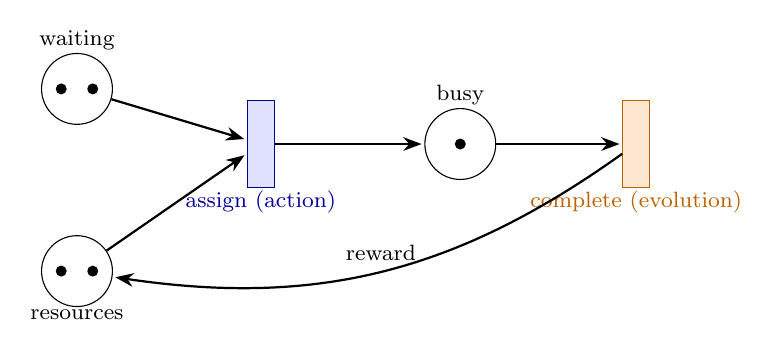
\begin{tikzpicture}[>=Stealth,node distance=1.5cm,
  place/.style={circle,draw,minimum size=9mm,inner sep=1pt},
  tok/.style={circle,fill=black,inner sep=1.4pt},
  act/.style={rectangle,draw=blue!60!black,fill=blue!12,minimum width=3.4mm,minimum height=11mm},
  evo/.style={rectangle,draw=orange!75!black,fill=orange!18,minimum width=3.4mm,minimum height=11mm},
  arc/.style={->,thick,shorten >=1pt},
  every label/.style={font=\footnotesize,inner sep=1pt}]
  \node[place,label=above:{\footnotesize waiting}] (w) {};
    \node[tok] at ([xshift=-2mm]w.center){}; \node[tok] at ([xshift=2mm]w.center){};
  \node[place,below=1.4cm of w,label=below:{\footnotesize resources}] (r) {};
    \node[tok] at ([xshift=-2mm]r.center){}; \node[tok] at ([xshift=2mm]r.center){};
  \node[act,right=1.7cm of w,yshift=-0.7cm,label=below:{\footnotesize\color{blue!60!black}assign (action)}] (a) {};
  \node[place,right=1.9cm of a,label=above:{\footnotesize busy}] (b) {};
    \node[tok] at (b.center){};
  \node[evo,right=1.6cm of b,yshift=0cm,label=below:{\footnotesize\color{orange!75!black}complete (evolution)}] (c) {};
  \draw[arc] (w) -- (a);
  \draw[arc] (r) -- (a);
  \draw[arc] (a) -- (b);
  \draw[arc] (b) -- (c);
  \draw[arc] (c) to[bend left=22] node[above,font=\footnotesize] {reward} (r);
\end{tikzpicture}
\caption{A minimal A-E PN for task assignment. Circles are places holding colored
tokens; bars are transitions. The \emph{assign} \textbf{action} transition
(blue) is a decision point: the policy chooses which waiting task to bind to which
free resource. The \emph{complete} \textbf{evolution} transition (orange) fires
automatically after a stochastic delay, returns the resource, and emits a reward.}
\label{fig:aepn}
\end{figure}

\paragraph{Policy gradient over A-E PN.} The policy $\pi_\theta$ is a graph neural
network over the assignment-graph representation \citep{aepn_repr2025}, trained
by PPO \citep{ppo2017} with generalized advantage estimation \citep{gae2016}. The
canonical unbiased gradient estimator credits each decision with its
reward-to-go against a learned baseline $V(s_d)$; both mechanisms below modify
only how that reward-to-go is computed.

% ======================================================================
\section{Method: two mechanisms, two affordances of the formalism}
\label{sec:method}

\paragraph{Two affordances, one formalism.} An A-E PN gives a learner two
things a black-box SMDP does not, and our two mechanisms exploit one each.
The first is \emph{token provenance}: a causal ancestry recorded for free by
the firing semantics, which \sccf{}/\ccf{} use to partition credit
(Section~\ref{sec:method:sccf}). The second is that the net is a
\emph{perfect, resettable forward model}: it can be snapshotted, forked and
replayed exactly, which \cfpk{} uses to measure a counterfactual directly
(Section~\ref{sec:method:cfpk}). We keep them separate deliberately. \cfpk{}
consults no provenance DAG at all---its coupling truncation is justified by a
state fingerprint (canonical marking plus clock), not by causal history---and
an ablation that \emph{adds} a lineage restriction to it is slightly worse on
the bottleneck environment. The two are complementary rather than variants of
one idea, and Section~\ref{sec:experiments} shows the complementarity is in
their coverage: provenance partitioning pays exactly where the problem
decomposes, and simulator replay pays where it does not.

\paragraph{Token provenance: the structure \sccf{} and \ccf{} exploit.} Each time
a transition fires we record which tokens it consumed and which it produced;
linking every produced token to the firing and the inputs that created it
yields the \emph{token-provenance DAG} (Figure~\ref{fig:prov}). Because in an
A-E PN every reward is a deterministic function of the tokens consumed at its
firing, this DAG contains the \emph{complete causal ancestry of every
reward}: walking backward from a reward reaches exactly the
tokens---and hence the action-decisions---that could have influenced it.
Formally, for reward $j$ let $\Ascr(j)\subseteq\{1,\dots,D\}$ be the set of
action-decisions reachable backward from $j$ in the DAG. This object requires
no additional modeling: it is implied by the net's firing semantics and
recorded at negligible cost during simulation. Prior A-E PN learning treats
the net as a black-box SMDP and never consults it.

\begin{figure}[t]
\centering
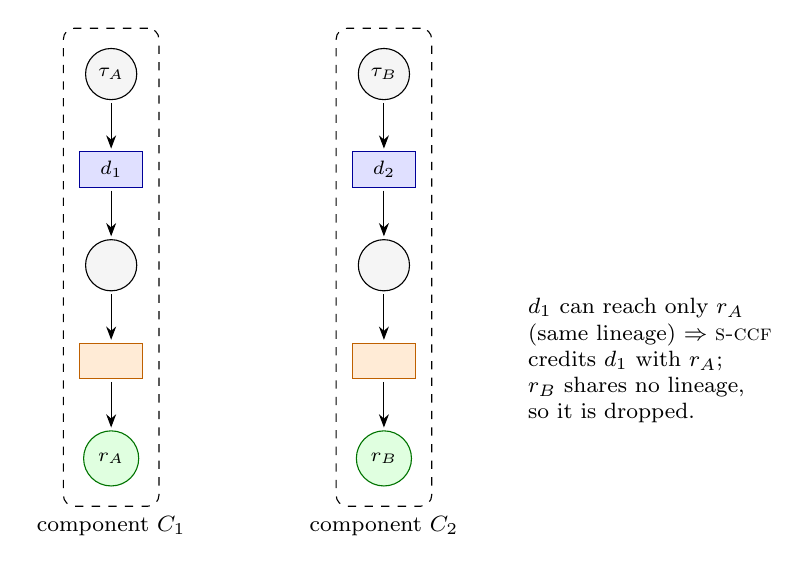
\begin{tikzpicture}[>=Stealth,node distance=6.5mm and 9mm,
  tok/.style={circle,draw,fill=gray!8,minimum size=6.5mm,inner sep=0pt,font=\scriptsize},
  fire/.style={rectangle,draw,fill=blue!12,draw=blue!60!black,minimum height=4.5mm,minimum width=8mm,font=\scriptsize},
  ev/.style={rectangle,draw,fill=orange!16,draw=orange!75!black,minimum height=4.5mm,minimum width=8mm,font=\scriptsize},
  rew/.style={circle,draw=green!45!black,fill=green!12,minimum size=7mm,inner sep=0pt,font=\scriptsize},
  a/.style={->,>=Stealth,shorten >=1pt,shorten <=1pt}]
  \node[tok] (tA) {$\tau_A$};
  \node[fire,below=of tA] (dA) {$d_1$};
  \node[tok,below=of dA] (bA) {};
  \node[ev,below=of bA] (eA) {};
  \node[rew,below=of eA] (rA) {$r_A$};
  \draw[a](tA)--(dA); \draw[a](dA)--(bA); \draw[a](bA)--(eA); \draw[a](eA)--(rA);
  \node[tok,right=2.8cm of tA] (tB) {$\tau_B$};
  \node[fire,below=of tB] (dB) {$d_2$};
  \node[tok,below=of dB] (bB) {};
  \node[ev,below=of bB] (eB) {};
  \node[rew,below=of eB] (rB) {$r_B$};
  \draw[a](tB)--(dB); \draw[a](dB)--(bB); \draw[a](bB)--(eB); \draw[a](eB)--(rB);
  \begin{scope}[on background layer]
    \node[draw,dashed,rounded corners,fit=(tA)(rA),inner sep=2.5mm,
          label=below:{\footnotesize component $C_1$}] {};
    \node[draw,dashed,rounded corners,fit=(tB)(rB),inner sep=2.5mm,
          label=below:{\footnotesize component $C_2$}] {};
  \end{scope}
  \node[align=left,font=\footnotesize,right=1.1cm of eB,xshift=2mm] {%
    $d_1$ can reach only $r_A$\\(same lineage) $\Rightarrow$ \textsc{s-ccf}\\
    credits $d_1$ with $r_A$;\\$r_B$ shares no lineage,\\so it is dropped.};
\end{tikzpicture}
\caption{Token provenance and causal components. Two cases flow through disjoint
resources, so their provenance never crosses: circles are tokens ($\tau$ tasks,
$r$ rewards), boxes are firings (blue = action decision $d_i$, orange =
evolution). Union-find over reward ancestries yields two components. A decision's
action can influence only rewards on its own lineage, so \sccf{} credits
$d_1$ with $r_A$ and drops the causally-unrelated $r_B$---whereas the full
reward-to-go (PPO) credits $d_1$ with $r_A+r_B$, injecting the variance of the
unrelated case.}
\label{fig:prov}
\end{figure}

\subsection{\sccf: causal-component-factored credit}
\label{sec:method:sccf}

\paragraph{A spectrum of credit signals.} Every redistribution scheme differs
only in \emph{which rewards each decision is allowed to see} (Table~\ref{tab:spectrum}).
The Monte-Carlo return \mcq{} credits a decision with \emph{all} future rewards;
it equals the PPO reward-to-go and is unbiased but high-variance. A
single-lineage restriction (\lrq) credits only rewards on the decision's own
token lineage; this cuts variance but is \emph{biased}, because it discards the
opportunity-cost rewards that sibling lineages---the roads not taken---would have
earned. \ccf{} keeps the whole \emph{realized} causal component, which fixes
\lrq's opportunity-cost bias but, as Section~\ref{sec:theory} shows, introduces a
different bias of its own at shared-resource handoffs. \sccf{} keeps the whole
\emph{static} causal component and is unbiased unconditionally.

\begin{table}[t]
\centering
\caption{The credit spectrum.}
\label{tab:spectrum}
\begin{tabular}{lccc}
\toprule
scheme & a decision sees\dots & bias & variance \\
\midrule
\mcq{} & all future rewards ($=$ PPO) & none & high \\
\lrq{} & its own token lineage & \textbf{biased} (opportunity cost) & low \\
\ccf{} & its own \emph{realized} causal component & \textbf{biased} (joins) & low \\
\sccf{} & its own \emph{static} causal component & none & low--moderate \\
\cfpk{} & exact forked counterfactual (no partition) & none & low (cost-bounded) \\
\bottomrule
\end{tabular}
\end{table}

\paragraph{Causal components via union-find.} For each reward $j$ we collect the
decisions in its lineage, $\Ascr(j)$, by a backward walk of the provenance DAG,
and union them: two decisions are placed in the same component whenever they
jointly caused a common reward. After processing all rewards, the decisions are
partitioned into causal components $C_1,\dots,C_M$; each reward with
$\Ascr(j)\neq\varnothing$ belongs to a well-defined component $c(j)$. In a
multi-copy system with disjoint resources this yields $M$ separate components;
when a shared resource links every case, freed resources re-enter the DAG and
$M=1$.

\paragraph{Component return-to-go.} Each decision $d$ (in component $c(d)$, at
clock $u_d$) is credited with the discounted rewards of its own component that
occur at or after $u_d$:
\begin{equation}
G_d^{\ccf} \;=\!\! \sum_{\substack{j:\,t_j\ge u_d\\ c(j)=c(d)}}\!\! \rho_d(t_j)\,r_j,
\qquad
G_d^{\mcq} \;=\!\! \sum_{j:\,t_j\ge u_d}\!\! \rho_d(t_j)\,r_j,
\end{equation}
and the advantage is $A_d = G_d^{\ccf}-V(s_d)$. The dropped quantity
$\Delta_d = G_d^{\mcq}-G_d^{\ccf}$ is the cross-component future reward.
Algorithm~\ref{alg:ccf} summarizes the computation; its cost is
$O(\text{decisions}\times\text{rewards})$ per episode, negligible next to the GNN
forward/backward passes. Postpone (wait) decisions, which under token-flow-off
have no reward-causing descendants, are handled by the standard SMDP temporal-
difference advantage rather than by this redistribution.

\paragraph{Action-dependent membership and the static fix (\sccf).} The union-find
above partitions decisions from the \emph{realized} trace, and that partition can
itself depend on the action taken. At an AND-join, a decision's choice determines
whether it merges with a joined decision's component, so a co-decision's private
reward enters its credit under one action but not the other---even though that
reward fires under both. The membership of \ccf's components is then
action-dependent, which (Section~\ref{sec:theory}) breaks the assumption behind
Proposition~\ref{prop:unbiased}: \ccf{} becomes biased at joins and can prefer a
suboptimal action (Section~\ref{sec:experiments} demonstrates an exact sign
flip). We therefore compute the component partition from the \emph{static net
topology} instead: two decisions share a component iff they \emph{could}
co-cause a reward under \emph{some} action sequence (topological reachability,
taking the union over a decision's competing actions). The resulting estimator,
\sccf, credits each decision with the realized rewards of its \emph{static}
component. Its membership is action-invariant by construction, so it is
unbiased without any assumption on the realized trajectory
(Proposition~\ref{prop:sccf}), while retaining \ccf's variance reduction on
statically-independent structure. On pure dynamic task assignment the two
coincide (assignment decisions create no joins); they diverge only at
synchronization transitions.

\paragraph{Which one is the method.} It is tempting to present \sccf{} alone,
since it is the variant with the unconditional guarantee. That would misdescribe
what the two estimators do. The static partition buys action-invariance by
being conservative, and on loosely-coupled problems it is conservative to the
point of being \emph{inert}: whenever any resource could in principle route
anywhere, $\Kstat=1$ and \sccf{} reduces to PPO exactly---which is the situation
on both of our non-constructed problems (multi-site routing and scaled
assignment; Section~\ref{sec:discussion}). \ccf{} is the estimator that acts
there, and it is the one carrying the empirical results of
Section~\ref{sec:experiments}.

We therefore present the two as a \emph{pair} spanning a bias/reach trade-off,
selected by the diagnostic of Section~\ref{sec:discussion}: \sccf{} where the
static partition already separates the problem, \ccf{} where only the realized
one does. The join bias is not hidden by this framing---it is the price of the
second column, we quantify it exactly (Table~\ref{tab:flip}), and we report that
we could not induce it in training across four purpose-built configurations.

\begin{algorithm}[t]
\caption{Causal-component-factored credit (\ccf{} / \sccf, differing only in
line~4)}
\label{alg:ccf}
\begin{algorithmic}[1]
\State \textbf{input:} episode trace with provenance DAG; decisions $1..D$; rewards $\{(r_j,t_j)\}$
\State initialize union-find over $\{1,\dots,D\}$
\For{each reward $j$ with $r_j\neq 0$}
  \State $\Ascr(j)\gets$ decisions reachable backward from $j$'s inputs in the DAG (\ccf: realized trace only; \sccf: static topology, union over competing actions)
  \State union all decisions in $\Ascr(j)$
\EndFor
\For{each decision $d$}
  \State $G_d\gets \sum_{j:\,c(j)=c(d),\,t_j\ge u_d} e^{-\beta(t_j-u_d)} r_j$
\EndFor
\State \textbf{return} advantages $A_d = G_d-V(s_d)$
\end{algorithmic}
\end{algorithm}

\subsection{\cfpk: simulator-replay counterfactual credit and coupling truncation}
\label{sec:method:cfpk}

The estimators above \emph{restrict} which realized rewards count toward a
decision's credit---a partition of a single trajectory. \cfpk{} takes a
different route: it does not partition anything. At a decision $d$ it forks
the simulator and replays the true environment dynamics forward under the
taken action $a_d$ and, separately, under an alternative $a_d'$, from the
identical pre-decision state---an exact, model-based counterfactual, since
the ``model'' is the real simulator (Section~\ref{sec:background}), not a
learned approximation.

\paragraph{Exact counterfactual credit.} For a branch $\omega\in\{a_d,a_d'\}$,
let $G_d(\omega)=\sum_{j:\,t_j\ge u_d}\rho_d(t_j)r_j^{(\omega)}$ be the
SMDP-discounted return realized by that branch's simulated continuation
(policy $\pi_\theta$ thereafter, to a lookahead horizon $L$ or episode end,
optionally closed off by a learned value-tail bootstrap at the horizon). The
credit signal is $I_d = G_d(a_d)-G_d(a_d')$: the exact realized counterfactual
advantage of the taken action, requiring no lineage partition and hence
immune to the shared-handoff bias that motivated \sccf.

\paragraph{Coupling truncation.} \cfpk's dominant cost is the fork itself: a
second full simulated continuation per decision. We reduce this, exactly and
for free, whenever the two branches' simulated states provably
\emph{reconverge}. Simulate both branches one environment step at a time in
lockstep, and let $\phi(\cdot)$ be a canonical, symmetry-collapsed
(marking, clock) state fingerprint (reused from an MCTS transposition-table
mechanism). If at round $\sigma$ the two branches' states coincide,
$\phi(s^{(a_d)}(\sigma))=\phi(s^{(a_d')}(\sigma))=:s^{*}$, decompose each
branch's return around $s^{*}$: $G_d(a_d)=P_{a_d}+\rho_d(t^{*})\tilde V(s^{*})$,
$G_d(a_d')=P_{a_d'}+\rho_d(t^{*})\tilde V(s^{*})$, where $P_\omega$ is branch
$\omega$'s own pre-reconvergence realized reward and $\tilde V(s^{*})$ is a
\emph{single} simulated continuation from $s^{*}$, reused for both branches
rather than drawn twice. Algorithm~\ref{alg:coupled} gives the lockstep
rollout; Proposition~\ref{prop:coupling} (Section~\ref{sec:theory}) proves the
shared term cancels exactly in $I_d$, so this is a strict cost reduction with
no correctness cost. If the branches never reconverge within the lookahead,
the mechanism falls back to two independent continuations---the
untruncated, always-exact base case.

\begin{algorithm}[t]
\caption{Coupling-truncated paired rollout (core of \cfpk)}
\label{alg:coupled}
\begin{algorithmic}[1]
\State \textbf{input:} snapshot at decision $d$; taken action $a_d$; alternative $a_d'$
\State fire $a_d$ and $a_d'$ from the snapshot, giving branches $A,B$ with running discounted totals $P_A,P_B$
\While{both $A,B$ active and within the lookahead}
  \If{$\phi(A)=\phi(B)$} \Comment{reconvergence: same canonical (marking, clock)}
    \State simulate ONE continuation $\tilde V$ from the shared state
    \State \Return $P_A+\tilde V,\; P_B+\tilde V$ \Comment{$\tilde V$ cancels exactly in the difference}
  \EndIf
  \State step $A$ and $B$ forward one environment step each, updating $P_A,P_B$
\EndWhile
\State \textbf{return} $P_A,P_B$ (no reconvergence: exact, untruncated two-branch rollout)
\end{algorithmic}
\end{algorithm}

\subsection{Positioning}
\label{sec:method:positioning}

Table~\ref{tab:spectrum} already positions the component-factored estimators and
\cfpk{} on the same bias/variance axis as \mcq/\lrq; the remaining axes are
\emph{reach} and \emph{cost}.

On reach, the two component-factored variants differ only in which partition
they use, and the diagnostic counts of Section~\ref{sec:discussion} say when
each has anything to work with: \sccf{} acts iff $\Kstat>1$, \ccf{} iff
$\Krea>1$, and $\Krea\ge\Kstat$ always. On cost, both are near-free---union-find
and component return-to-go are negligible next to the GNN passes---whereas
\cfpk{} is exact and fine-grained at \emph{every} decision, including
synchronization points where neither partition helps, at a bounded extra cost
from forking, one proven and free chunk of which coupling truncation removes.

This gives three regimes rather than two, and Section~\ref{sec:discussion}
turns them into a decision rule: use \sccf{} when the static partition already
separates the problem, \ccf{} when only the realized one does, and \cfpk{} when
neither does but the extra simulation budget is available.

% ======================================================================
\section{Theoretical analysis}
\label{sec:theory}

\subsection{\sccf: unbiasedness and variance reduction}
\label{sec:theory:sccf}

We take as given that the full reward-to-go estimator is unbiased,
$\Ex[\hat g^{\mcq}]=\nabla_\theta J(\theta)$ \citep{sutton2000pg}; all statements
are relative to it. Let $\Fscr_d$ denote the history up to but excluding $a_d$.

\begin{assumption}[Component mean-exogeneity]\label{ass:a1}
For every decision $d$, $\;\Ex[\Delta_d\mid \Fscr_d, a_d] = \Ex[\Delta_d\mid \Fscr_d]$.
\end{assumption}

Assumption~\ref{ass:a1} holds by A-E PN semantics: a reward is a deterministic
function of the tokens it consumes, whose full history is recorded, so $a_d$ can
influence $r_j$ only if some descendant of $a_d$ lies on $j$'s lineage---i.e.\
only if $c(j)=c(d)$. Cross-component rewards therefore have no causal path from
$a_d$; the only residual channel is the exogenous randomness driving other
components' events, which is independent of $a_d$ under the standard model of
independent per-firing draws.

\begin{proposition}[Unbiasedness]\label{prop:unbiased}
Under Assumption~\ref{ass:a1}, $\;\Ex[\hat g^{\ccf}]=\Ex[\hat g^{\mcq}]=\nabla_\theta J(\theta)$.
\end{proposition}
\begin{proof}
The estimators differ only through $\Delta_d$:
$\hat g^{\mcq}-\hat g^{\ccf}=\sum_d \nabla_\theta\log\pi_\theta(a_d\mid s_d)\,\Delta_d$.
Conditioning on $\Fscr_d$ and drawing $a_d\sim\pi_\theta(\cdot\mid s_d)$,
\[
\Ex\!\left[\nabla\log\pi_\theta(a_d\mid s_d)\,\Delta_d \mid \Fscr_d\right]
=\Ex_{a_d}\!\left[\nabla\log\pi_\theta(a_d\mid s_d)\,\Ex[\Delta_d\mid \Fscr_d,a_d]\right].
\]
By Assumption~\ref{ass:a1} the inner expectation equals
$\bar\Delta_d:=\Ex[\Delta_d\mid\Fscr_d]$, independent of $a_d$, so the expression
is $\bar\Delta_d\,\Ex_{a_d}[\nabla\log\pi_\theta(a_d\mid s_d)]=\bar\Delta_d\,\nabla_\theta\!\sum_a\pi_\theta(a\mid s_d)=0$.
Summing over $d$ gives $\Ex[\hat g^{\mcq}-\hat g^{\ccf}]=0$.
\end{proof}

\begin{proposition}[Variance reduction]\label{prop:var}
Suppose at decision $d$ the future reward-to-go splits across $K$ causally-
independent components, $G_d^{\mcq}=\sum_{k=1}^{K}R_k$ with $d$ in component $1$
and $G_d^{\ccf}=R_1$, and that conditional on $s_d$ the $R_k$ are mutually
independent with variances $\sigma_k^2$. Then, for the mean baseline
$V(s_d)=\Ex[G_d^{\mcq}\mid s_d]$,
\[
\Var(G_d^{\mcq}-V\mid s_d)=\textstyle\sum_{k=1}^K\sigma_k^2,
\qquad
\Var(G_d^{\ccf}-V\mid s_d)=\sigma_1^2.
\]
If $\sigma_k^2\approx\sigma^2$, \ccf{} reduces per-decision advantage variance by
a factor $\approx K$ (gradient-noise standard deviation by $\approx\sqrt K$).
\end{proposition}
\begin{proof}
Immediate from independence: $\Var(\sum_k R_k)=\sum_k\sigma_k^2$; subtracting the
$s_d$-measurable constant $V$ leaves variances unchanged; and $G_d^{\ccf}=R_1$.
\end{proof}

\begin{corollary}[Monotone variance reduction]\label{cor:mono}
Assume only that, conditional on $s_d$, $G_d^{\ccf}$ and $\Delta_d$ are
uncorrelated (implied by causal independence of distinct components). Then for
\emph{any} baseline $V(s_d)$,
\[
\Var(G_d^{\mcq}-V\mid s_d)=\Var(G_d^{\ccf}-V\mid s_d)+\Var(\Delta_d\mid s_d)
\;\ge\;\Var(G_d^{\ccf}-V\mid s_d),
\]
with equality iff $\Var(\Delta_d\mid s_d)=0$ (in particular whenever $M=1$).
\end{corollary}
\begin{proof}
Write $G_d^{\mcq}-V=(G_d^{\ccf}-V)+\Delta_d$; expand the variance; the cross term
is $\Cov(G_d^{\ccf},\Delta_d\mid s_d)=0$ by assumption. Nonnegativity of
$\Var(\Delta_d)$ gives the inequality.
\end{proof}

Corollary~\ref{cor:mono} is the robust statement: \ccf{} is \emph{never worse}
than PPO in advantage variance, for any critic and with no assumption on the
number of components, and strictly better wherever cross-component reward exists.
When a shared resource collapses the system to one component ($M=1$),
$\Delta_d\equiv0$ and \ccf{} is identically PPO---the honest null we confirm
empirically and build on directly in Section~\ref{sec:boundary}.

\paragraph{When Assumption~\ref{ass:a1} fails, and \sccf.} Assumption~\ref{ass:a1}
treats the component partition as fixed, but \ccf{} reads it from the realized
trace, and the partition can depend on $a_d$. At an AND-join, action $A$ fires
the join and merges $d$ with a co-decision $d'$ (so $d'$'s private reward
$r'\in c(d)$), while action $B$ does not ($r'\notin c(d)$); yet $r'$ fires under
both. Hence $\Ex[\Delta_d\mid\Fscr_d,a_d]$ depends on $a_d$: Assumption~\ref{ass:a1}
fails, and with $r'>r_1-r_{\text{join}}$ the sign of $d$'s credit difference
reverses, so \ccf{} prefers the suboptimal join (Section~\ref{sec:experiments}
gives an exact numerical instance). The remedy is to make membership
action-invariant.

\begin{assumption}[Static membership]\label{ass:a1p}
The component partition is a function of the net topology alone: two decisions
share a component iff they can co-cause a reward under \emph{some} action
sequence. In particular it does not depend on $a_d$.
\end{assumption}

\begin{proposition}[Unbiasedness of \sccf]\label{prop:sccf}
Under Assumption~\ref{ass:a1p}, the rewards \sccf{} drops
($\{r_j:c(j)\neq c(d)\}$) are, by topological construction, unreachable from
$a_d$ under any action, hence action-independent given $s_d$. The argument of
Proposition~\ref{prop:unbiased} then applies verbatim with Assumption~\ref{ass:a1p}
in place of Assumption~\ref{ass:a1}: $\Ex[\hat g^{\sccf}]=\nabla_\theta J(\theta)$,
with no assumption on the realized trajectory.
\end{proposition}

\sccf{} thus \emph{dominates} \ccf: unbiased in the join and shared-handoff
regimes where \ccf{} (and \lrq) can flip to a suboptimal action, and identical to
\ccf{} on pure task assignment, where assignment decisions create no joins. We
establish the bias and the fix at the estimator level
(Section~\ref{sec:experiments}); a clean training-level demonstration of the
\ccf{} flip is elusive, because the very structure that triggers it---a private
reward coupled through a join---is an intrinsically hard credit-assignment
problem in which even the unbiased baseline (PPO) fails to reach the optimum.

\subsection{\cfpk: coupling truncation is exact}
\label{sec:theory:cfpk}

\begin{assumption}[Fingerprint sufficiency]\label{ass:a3}
For any two simulated states $s,s'$ with $\phi(s)=\phi(s')$, the conditional
law of all future (policy and exogenous) randomness given $s$ equals that
given $s'$: $\phi$ is a bisimulation-consistent sufficient statistic for the
SMDP's transition-and-reward kernel.
\end{assumption}

Assumption~\ref{ass:a3} holds by construction: the AEPN's dynamics depend on
the marking and the clock alone, and $\phi$ discards nothing but token
identities within a class of tokens that are, by construction, interchangeable
in every downstream rule (same place, same attributes, same enabled
transitions).

\begin{proposition}[Coupling truncation is exact]\label{prop:coupling}
Under Assumption~\ref{ass:a3}, for any realization of the pre-reconvergence
randomness, the coupling-truncated credit signal satisfies
$I_d^{\text{coupled}}=G_d(a_d)-G_d(a_d')=P_{a_d}-P_{a_d'}$ exactly---the
shared continuation $\tilde V(s^{*})$ cancels identically, regardless of its
realized value. Consequently $I_d^{\text{coupled}}$ targets the same quantity
as the naive estimator that draws two independent continuations from
$s^{*}$, and has strictly lower variance whenever $\Var(\tilde V(s^{*})\mid
s^{*})>0$: the reconverged tail contributes exactly zero variance to
$I_d^{\text{coupled}}$, versus $\rho_d(t^{*})^2\cdot 2\Var(\tilde V(s^{*})\mid
s^{*})$ (two independent draws) to the naive estimator.
\end{proposition}
\begin{proof}
\emph{Exact cancellation.} Immediate from the decomposition: the
$\rho_d(t^{*})\tilde V(s^{*})$ term is the same real number added to both
$G_d(a_d)$ and $G_d(a_d')$, so it cancels in the difference for every
realization---no appeal to Assumption~\ref{ass:a3} is needed for this half,
only that the implementation reuses one draw.
\emph{Same target.} Assumption~\ref{ass:a3} gives that both branches'
post-$\sigma$ continuations are drawn from the identical distribution with
mean $V^{\pi}(s^{*})$, so the naive estimator's cross term has expectation
$\rho_d(t^{*})(V^{\pi}(s^{*})-V^{\pi}(s^{*}))=0$: both estimators target
$\Ex[P_{a_d}-P_{a_d'}]$.
\emph{Variance.} The naive estimator's two continuation draws are simulated
independently of each other and of the pre-$\sigma$ randomness (Markov
property), so its variance is $\Var(P_{a_d}-P_{a_d'})+\rho_d(t^{*})^2\cdot
2\Var(\tilde V(s^{*})\mid s^{*})$, while $I_d^{\text{coupled}}=P_{a_d}-P_{a_d'}$
exactly, giving $\Var(I_d^{\text{coupled}})=\Var(P_{a_d}-P_{a_d'})$---strictly
smaller whenever the reconverged tail has any variance at all.
\end{proof}

This is a stronger claim than a typical common-random-numbers coupling
argument, which \emph{reduces} shared-tail variance by inducing positive
correlation between two draws; here the shared draw is not merely correlated
across branches, it \emph{is} the same draw, so the tail's contribution to
the paired difference is not reduced but eliminated. Unlike CRN, this needs
no alignment of the two branches' random-number-stream \emph{positions} at
reconvergence---only that they have reached the same \emph{state}, which
Assumption~\ref{ass:a3} guarantees determines the same future distribution
regardless of how each branch got there. \emph{(Full remarks---no-RNG-alignment
detail, agnosticism to the value-tail-bootstrap procedure, the lineage-mode
scope gate---in the appendix.)}

% ======================================================================
\section{Experiments}
\label{sec:experiments}

We answer six questions. \textbf{Q1:} Does \sccf{} reduce to PPO when the
system is a single causal component (correctness)? \textbf{Q2:} Does \sccf{}
beat PPO as concurrent independence grows? \textbf{Q3:} Does the win hold on a
realistic operational problem? \textbf{Q4:} Is the win attributable to the
\emph{component factoring} specifically, rather than to the SMDP
return-to-go machinery it is built on? \textbf{Q5:} Does \ccf's bias mechanism
manifest concretely, and does \sccf{} fix it? \textbf{Q6:} Is coupling
truncation exact, and does it measurably reduce \cfpk's cost, at real
training scale?

\paragraph{Protocol.} The baseline is PPO with SMDP-matched discounting, so the
\emph{only} difference from \sccf{}/\ccf{} is the credit factoring. Returns are
normalized so that $0$ is a random policy and $1$ a strong domain heuristic. We
report means with $95\%$ confidence intervals over independent seeds and test
significance with Welch's $t$ and Mann--Whitney $U$.

\paragraph{The lineage ablation (Q4).} PPO is the right baseline for ``does
credit factoring help'', but it cannot separate the \emph{factoring} from the
per-decision SMDP return-to-go the factored schemes are built on. We therefore
add \mcq{} as an explicit \emph{lineage ablation}: the identical estimator with
the causal-component test deleted, so each decision receives the full
discounted return-to-go from its own clock. \ccf{} minus \mcq{} isolates the
contribution of the decomposition itself, and is the comparison we report
alongside \ccf{} minus PPO throughout.

\paragraph{Mechanism (Q2, Figure~\ref{fig:mech}).} On $N$ causally-independent
copies of a base assignment task, the divergence between \ccf{} and PPO credit,
$|\ccf-\mcq|/\text{scale}$, rises monotonically from $0.09$ ($N{=}1$) to $0.84$
($N{=}8$): more independent components means more concurrent-case noise for
\ccf{} to factor away, exactly as Proposition~\ref{prop:var} predicts.

\paragraph{Scaling (Q1--Q2, Figure~\ref{fig:scaling}).} Training on the same
family, \ccf{} and PPO are statistically tied at $N{=}1$ (one component, nothing
to factor---the required null), while for $N>1$ \ccf{} holds near the optimum and
PPO degrades and destabilizes (its seed-to-seed variance balloons; individual
seeds finish at or below the random baseline). \ccf{} exhibits
\emph{stable optimality} where PPO exhibits \emph{credit-collapse}. (These
topologies have no shared-resource handoff, so \ccf{} and \sccf{} coincide
exactly here---see the note following Table~\ref{tab:flip}.)

\paragraph{Realistic operational problem (Q3, Figure~\ref{fig:multisite}).} We
model multi-site skills-based routing: $n_{\text{sites}}$ service sites, each with
its own arrival stream and a heterogeneous pool of local specialists, plus a
shared pool of flexible generalists---the classic resource pooling/flexibility
setting \citep{pooling_flexibility}. In the independent-site configuration
($n_{\text{sites}}{=}4$, $12$ seeds, $40$ epochs), PPO \emph{fails to learn} the
routing: its learning curve is flat and it plateaus at normalized return $0.15$
(median $0.06$; $2/12$ seeds exceed $0.5$). \ccf{} learns it, rising to $0.52$
(median $0.55$; $6/12$ seeds exceed $0.5$). The difference is significant
(Welch $p=0.005$, Mann--Whitney $p=0.004$) with a large effect size (Cohen's
$d=1.27$) and disjoint $95\%$ CIs (Table~\ref{tab:multisite}).

\begin{table}[t]
\centering
\caption{Multi-site skills-based routing (independent config, $4$ sites, $12$
seeds, $40$ epochs). Normalized greedy return.}
\label{tab:multisite}
\begin{tabular}{lccc}
\toprule
method & norm.\ final (95\% CI) & median & seeds $>0.5$ \\
\midrule
PPO (discount-matched) & $0.146 \pm 0.150$ & $0.058$ & $2/12$ \\
\mcq{} (lineage ablation) & $0.036 \pm 0.121$ & $0.068$ & $0/12$ \\
\ccf{} (ours)          & $\mathbf{0.518 \pm 0.181}$ & $0.546$ & $6/12$ \\
\bottomrule
\end{tabular}
\end{table}

\paragraph{The win is the factoring, not the return-to-go (Q4,
Table~\ref{tab:ablation}).} Running the \mcq{} lineage ablation on both
families settles what PPO comparisons cannot. On the $N$-copies sweep the
ablation tracks \ccf{} while independence is scarce and then falls away from it:
at $N{=}8$, \mcq{} is statistically indistinguishable from PPO
($+0.005$, $p=0.97$) while \ccf{} is $+0.564$ above \mcq{} ($12/12$ seeds,
$p=0.0001$). In other words the \emph{entire} margin over PPO at $N{=}8$ is the
component decomposition; the SMDP return-to-go contributes none of it. Multi-site
routing replicates this on a non-constructed problem: \mcq{} reaches $0.036$,
\emph{below} PPO's $0.146$, while \ccf{} is $+0.482$ above \mcq{}
($11/12$ seeds, $p=0.0005$).

\begin{table}[t]
\centering
\caption{Lineage ablation (Q4). \mcq{} is \ccf{} with the causal-component test
deleted, so $\ccf-\mcq$ isolates the decomposition. Normalized greedy return;
$12$ seeds throughout; $p$ from a paired $t$-test on shared seeds.}
\label{tab:ablation}
\begin{tabular}{lccccc}
\toprule
problem & $K$ & PPO & \mcq{} & \ccf{} & $\ccf-\mcq$ \\
\midrule
$N$-copies, $N{=}1$ & $1$ & $0.864$ & $0.895$ & $0.893$ & $-0.003$ \hfill ($p{=}0.90$) \\
$N$-copies, $N{=}2$ & $2$ & $0.319$ & $0.517$ & $0.654$ & $+0.137$ \hfill ($p{=}0.56$) \\
$N$-copies, $N{=}4$ & $4$ & $0.523$ & $0.692$ & $0.796$ & $+0.105$ \hfill ($p{=}0.43$) \\
$N$-copies, $N{=}8$ & $8$ & $0.362$ & $0.367$ & $\mathbf{0.931}$ & $\mathbf{+0.564}$ \hfill ($p{=}0.0001$) \\
multi-site routing  & $12^{\dagger}$ & $0.146$ & $0.036$ & $\mathbf{0.518}$ & $\mathbf{+0.482}$ \hfill ($p{=}0.0005$) \\
\bottomrule
\end{tabular}

\smallskip
\footnotesize $^{\dagger}$ realized component count; the \emph{static} count is
$1$ on this problem---see Section~\ref{sec:discussion}.
\end{table}

Two cautions on reading Table~\ref{tab:ablation}. The intermediate gaps at
$N{=}2$ and $N{=}4$ are \emph{not} significant ($p=0.56$, $0.43$): the evidence
for the decomposition is carried by $N{=}8$ and by multi-site, not by a fitted
trend across four points. And the $\ccf-\mcq$ column is flat until independence
is genuinely present and then large, which is the qualitative shape
Proposition~\ref{prop:var} predicts, but we do not claim a scaling law from it.

\paragraph{Cost (Q2--Q3).} Measured \ccf{}/PPO wall-clock is $\approx1.0\times$
across the sweeps (at the largest size \ccf{} was in fact faster): the
union-find and component return-to-go are negligible next to the GNN passes.

\paragraph{The \ccf{} bias, exactly (Q5, Table~\ref{tab:flip}).} On a
deterministic shared-resource join motif (decision $d_1$: consume a shared
resource now, delaying a second stream's private reward, versus leave it
free; $\beta=0.3$), we compare each scheme's $d_1(A{-}B)$ credit difference
against \mcq's, which is exact on a deterministic trace and hence the ground
truth for which action is optimal.

\begin{table}[t]
\centering
\caption{Shared-resource join motif, $\beta=0.3$. \mcq{} is the unbiased
ground truth on this deterministic trace; \ccf{} and \lrq{} flip sign
(prefer the suboptimal action); \sccf{} recovers the exact value.}
\label{tab:flip}
\begin{tabular}{lcl}
\toprule
scheme & $d_1(A-B)$ & verdict \\
\midrule
\mcq{} (ground truth) & $-7.606$ & optimal action $=B$ \\
\lrq{} & $+2.394$ & \textbf{FLIP} $\to$ suboptimal \\
\ccf{} & $+2.394$ & \textbf{FLIP} $\to$ suboptimal \\
\sccf{} & $-7.606$ & unbiased, exact \\
\bottomrule
\end{tabular}
\end{table}

\ccf{} and \lrq{} not only lose magnitude, they reverse sign: both would
select the suboptimal action. \sccf{} recovers the ground truth exactly, on
this and every instance of the motif we tested. On topologies with no
shared-resource handoff (the $N$-copies and independent-site multi-site
configurations above), realized and static partitions coincide exactly, so
the \ccf{} numbers reported for Q1--Q3 are precisely what \sccf{} would have
produced there; this equivalence does not extend to topologies with genuine
handoffs, which is exactly what Table~\ref{tab:flip} isolates.

\paragraph{Coupling truncation: exactness and cost (Q6).} On a controlled
net built to guarantee reconvergence after a corridor of decisions, coupling
truncation reduces simulated \texttt{env.step} calls from $18$ to $12$
($33\%$) with paired gap/standard-error numerically \emph{identical}
with/without truncation, confirming Proposition~\ref{prop:coupling}'s
exactness claim directly in the implementation. At real training scale, on a
contested/joint topology chosen to fork often (full protocol: $30$ epochs
$\times$ $20$ episodes/epoch, $12$ seeds), coupling truncation gives a
$1.37\times$ wall-clock speedup ($36.25\to26.53$ minutes/cell) with
\texttt{norm\_final} \emph{exactly identical} ($1.000$ vs.\ $1.000$) across all
$12$ seeds (Table~\ref{tab:coupling})---the zero-variance-contribution property of
Proposition~\ref{prop:coupling} predicts precisely this outcome: no change to
what is learned, only to how it is computed.

\begin{table}[t]
\centering
\caption{Coupling truncation, real training scale (contested/joint topology,
$30$ epochs $\times$ $20$ episodes/epoch, $12$ seeds).}
\label{tab:coupling}
\begin{tabular}{lccc}
\toprule
& minutes/cell & speedup & norm.\ final \\
\midrule
\cfpk{} without coupling truncation & $36.25$ & --- & $1.000$ \\
\cfpk{} with coupling truncation & $26.53$ & $\mathbf{1.37\times}$ & $1.000$ \\
\bottomrule
\end{tabular}
\end{table}

\begin{figure}[t]
\centering
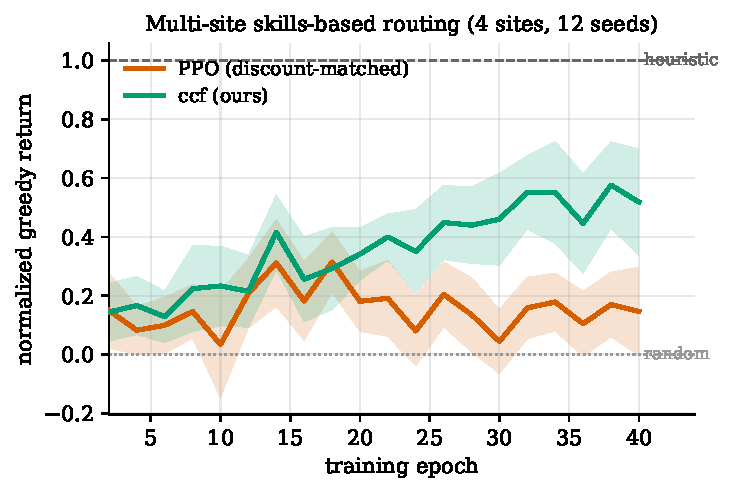
\includegraphics[width=0.7\linewidth]{../figures/fig1_multisite_curves.pdf}
\caption{Realistic multi-site skills-based routing ($12$ seeds, $95\%$ CI bands).
PPO plateaus (does not learn the routing); \ccf{} learns it and keeps rising.}
\label{fig:multisite}
\end{figure}

\begin{figure}[t]
\centering
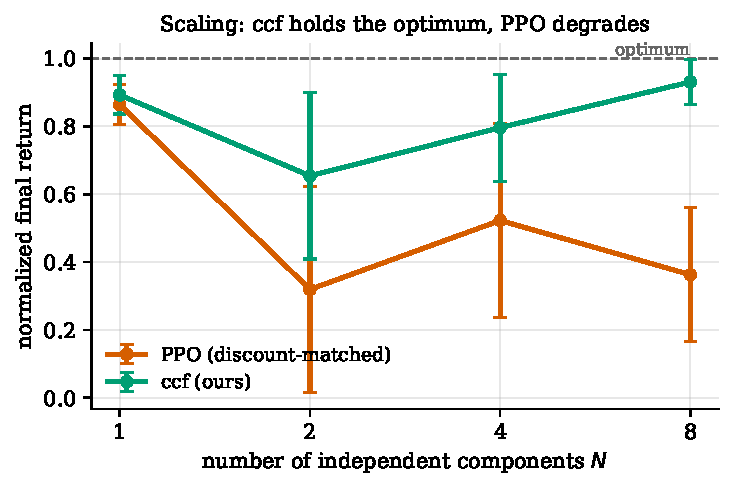
\includegraphics[width=0.7\linewidth]{../figures/fig2_ncopies_scaling.pdf}
\caption{Scaling with the number of independent components $N$. \ccf{} holds the
optimum; PPO degrades and destabilizes. Tied at $N{=}1$ (the null).}
\label{fig:scaling}
\end{figure}

\begin{figure}[t]
\centering
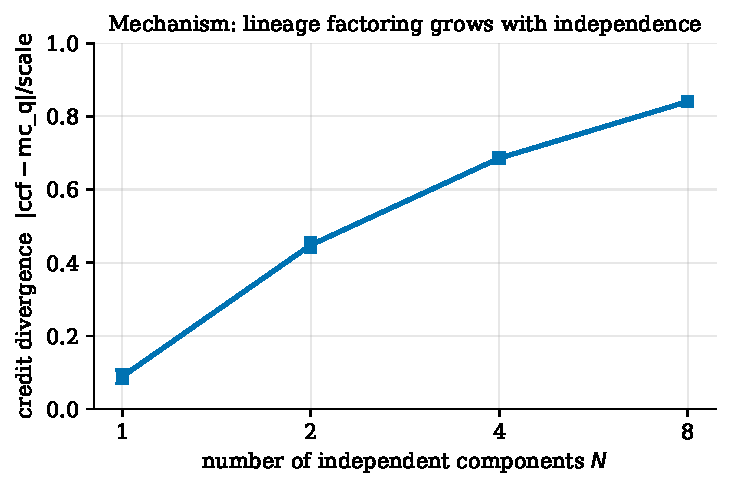
\includegraphics[width=0.7\linewidth]{../figures/fig3_mechanism_factoring.pdf}
\caption{Mechanism: the divergence between \ccf{} and PPO credit grows with the
number of independent components, as Proposition~\ref{prop:var} predicts.}
\label{fig:mech}
\end{figure}

% ======================================================================
\section{The boundary-condition investigation}
\label{sec:boundary}

Corollary~\ref{cor:mono} makes a sharp prediction: \sccf's variance reduction
scales with the number of causally independent components $K$, and collapses
to \emph{exactly} PPO when $K=1$ (a single shared resource pool links every
case into one component). This is the theorem's own honest null, not a
failure. We use a two-stage service-line environment with a single shared,
skill-heterogeneous employee pool (henceforth the \emph{bottleneck
environment}) as the decisive $K{=}1$ case, and ask: can the residual gap on
this genuinely single-component problem be closed by any other provenance- or
structure-based route? We tested three independent, well-motivated
candidates---never touching credit, only what the learner observes---and
found each provably inert or empirically neutral. Table~\ref{tab:boundary}
summarizes; we report all three not as a coda but as a result, since two of
the three failures follow from a proof rather than a correlation and
together they localize the bottleneck's difficulty precisely.

\paragraph{Reward shaping.} Potential-based shaping from PN topology
\citep{ng1999shaping}, SMDP-generalized, is provably policy-invariant for any
potential function---verified directly in code via an exact terminal-value
cancellation test, not merely cited. A full coefficient dial on the
bottleneck environment (same cached PPO baseline reused across all four
points) shows reach-rate cleanly monotonic in the injected-variance
direction ($8/10\to4/10\to1/10$ seeds reaching $95\%$ of the heuristic
anchor as the coefficient rises $0.2\to0.5\to1.0$), and no coefficient
produces a significant win: $0.739\pm0.10$ (baseline) vs.\ $0.766\pm0.10$
($p=.48$, coefficient $0.2$) vs.\ $0.420\pm0.10$, $0$W/$10$L (coefficient
$1.0$). The mechanism is that constant exogenous arrivals make the potential
rise as well as fall, injecting a per-step signal on the same order of
magnitude as the full episode return---unbiased in aggregate (guaranteed by
the theorem) but a substantially noisier value-regression target at a finite
budget.

\paragraph{Structural input features.} Static, conflict-graph-derived scalars
appended to each action node's own input features (does this action type
structurally compete for a token, and with how many; and, after a first null
result, the minimum topological distance to the nearest reward among an
action's required inputs) are both statistically neutral ($p=.58$ and
$p=.69$ respectively). The stronger finding is \emph{why}: every action node
already carries a one-hot action-type identity at zero hops, so the two
competing action types in the bottleneck environment are already fully
distinguishable with or without any structural feature. Any scalar computed
as a function of action type alone is therefore a deterministic function of
information a single learned weight on the one-hot could already
reconstruct---provably redundant, not merely observed to be unhelpful across
two experiments, and true of this architecture on any topology, not only the
bottleneck environment.

\paragraph{Actor architecture.} We identify and prove a previously
undocumented limitation: the actor decodes each action's logit from only that
action node's own final message-passing embedding, unlike the critic, which
has always pooled over all action/postpone node embeddings for its value
estimate. Combined with graph edges directed strictly along token flow (no
reverse edges at any real observation call site), an action's logit can
depend on state only via a forward path reaching it within the network's
depth. We prove this is a hard architectural fact, not a training-budget
limitation: on a purpose-built topology of two structurally independent
two-stage pipelines, perturbing one pipeline's downstream marking left the
other pipeline's action logit \emph{exactly, bit-for-bit unchanged} under a
randomly initialized, untrained network ($\Delta=0.000$)---reachability is a
property of the computational graph, independent of learned weights. We fix
this (concatenating the same pooled context the critic already computes onto
each action node before decoding), confirm the fix closes the gap on the
same proof topology ($\Delta=0.000\to0.528$), and re-test on the bottleneck
environment: norm.\ final $0.739\pm0.10$ (baseline) vs.\ $0.746\pm0.14$
(fixed architecture), $p=.91$---no significant effect. The proof and the
training result are not in tension: the bottleneck environment's shared
resource pool happens to recycle, giving the unfixed architecture a
marginal, accidental backdoor to the same information, so the blind spot was
never total there, and whatever fraction the fix newly exposes is not, in
practice, decision-relevant enough to move a well-tuned baseline at this
training budget.

\begin{table}[t]
\centering
\caption{The boundary-condition investigation, bottleneck environment
($K{=}1$).}
\label{tab:boundary}
\begin{tabular}{lll}
\toprule
mechanism & theoretical status & result \\
\midrule
Reward shaping & policy-invariant, any potential & neutral (0.2) to harmful (1.0), $0$W/$10$L \\
Structural input features & mechanically correct & neutral, $p=.58\to.69$; provably redundant \\
Actor global context & proven to close a real gap & neutral, $p=.91$; gap was already marginal here \\
\bottomrule
\end{tabular}
\end{table}

\begin{figure}[t]
\centering
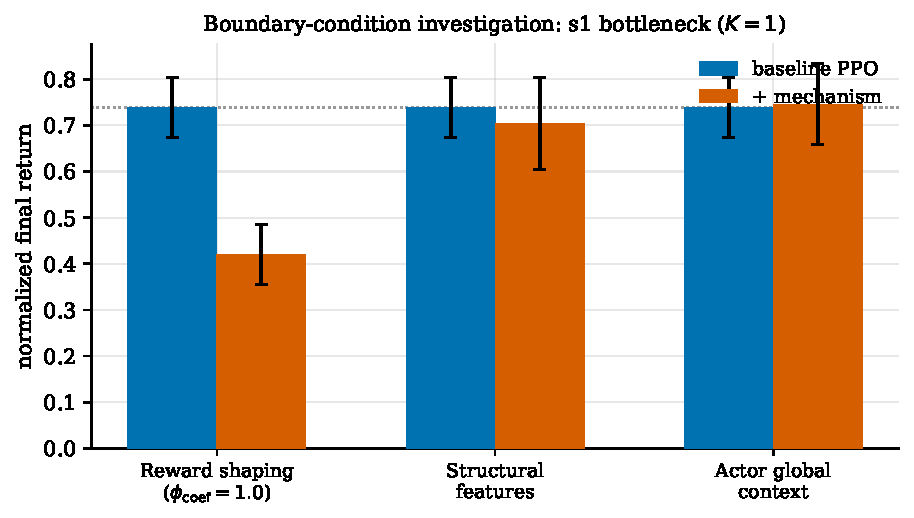
\includegraphics[width=0.78\linewidth]{../figures/fig4_boundary_summary.pdf}
\caption{Baseline PPO vs.\ each of the three boundary-condition mechanisms on
the bottleneck environment ($K{=}1$; error bars are $95\%$ CIs over seeds).
None significantly improves on the baseline; reward shaping at
$\phi_{\mathrm{coef}}{=}1.0$ is significantly worse.}
\label{fig:boundary}
\end{figure}

\begin{figure}[t]
\centering
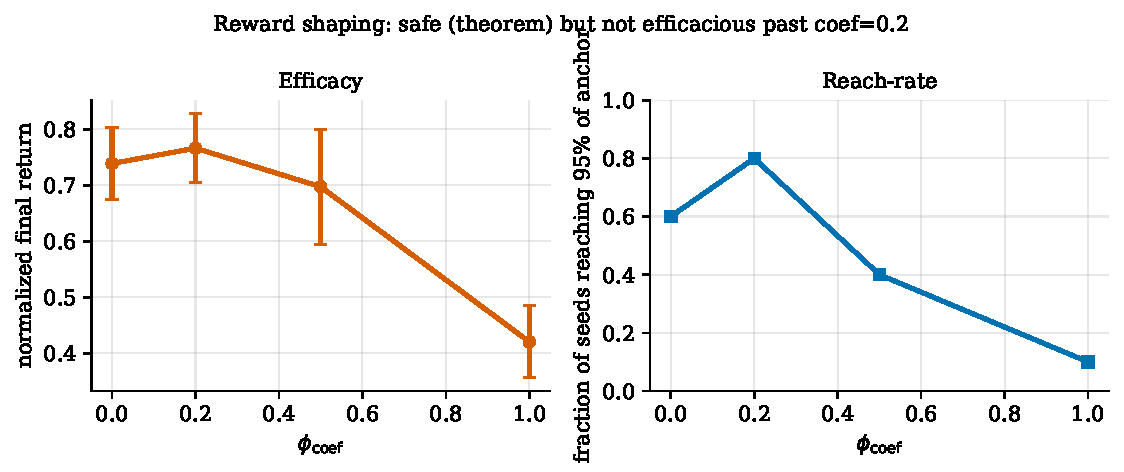
\includegraphics[width=\linewidth]{../figures/fig5_phi_dial.pdf}
\caption{The reward-shaping coefficient dial on the bottleneck environment:
efficacy (left) degrades once past $\phi_{\mathrm{coef}}=0.2$, and the
fraction of seeds reaching $95\%$ of the heuristic anchor (right) degrades
monotonically---safety (Section~\ref{sec:related}, \citealp{ng1999shaping})
and efficacy are independent properties, and this mechanism has the first
without the second at practical training budgets.}
\label{fig:phidial}
\end{figure}

None of this is a failure of experimental design: each mechanism does
exactly what it was built to do. It is evidence about where the bottleneck
environment's difficulty does \emph{not} live---not in what the learner can
observe, and not, per Corollary~\ref{cor:mono}, in an avoidable credit bias
on this genuinely single-component topology. We state this as an open
problem rather than a solved one in Section~\ref{sec:discussion}.

% ======================================================================
\section{Discussion}
\label{sec:discussion}

\paragraph{A decision rule, not just a result.} The causal-component
count $K$ (Proposition~\ref{prop:var}) is computed automatically, as a
byproduct of the same union-find machinery the credit mechanism already
runs, from a handful of simulated episodes under any reasonable policy---a
concrete, pre-training diagnostic. If $K>1$ reliably, the mechanisms in this
paper apply, and the choice between them is a cost/granularity
trade-off (below). If $K\approx1$ essentially always---most commonly one
shared, fully-utilized resource pool---neither mechanism will outperform a
well-tuned PPO baseline, and Section~\ref{sec:boundary} gives three
independently verified reasons not to expect a workaround from adjacent
directions either. Concretely: parallel production lines, multiple sites or
service branches, and segmented (even loosely) resource pools are exactly
the structures that produce $K>1$; a single, centrally pooled team or
machine bank serving one undifferentiated queue is exactly the structure
that collapses to $K=1$. Many real operations sit continuously in between,
and the diagnostic handles this directly.

\paragraph{Two counts, and they select between the two variants.} $K$ is not a
single number: the diagnostic returns a \emph{static} and a \emph{realized}
count, and the gap between them is what chooses \sccf{} over \ccf{}.
$\Kstat$ partitions on topology---two decisions share a component if they
\emph{could ever} reach a common reward---so it is conservative and
action-invariant, which is precisely the property that makes \sccf{}
unbiased (Section~\ref{sec:theory}). $\Krea$ partitions on the realized
provenance DAG, merging only decisions that \emph{did} touch a common reward;
it is finer, and it is what \ccf{} uses.

The two can differ sharply, and they differ most on exactly the problems one
cares about. On multi-site routing $\Kstat=1$---a single shared pool of
flexible generalists could in principle couple every site to every other---while
$\Krea=12$, because in practice the sites are served locally and rarely
interact. The same pattern holds on the scaled single-stage assignment problem
($\Kstat=1$, $\Krea=6$). Where the two agree, the variants coincide: on the
$N$-copies family both equal $N$, and \sccf{} and \ccf{} are identical there.

The practical rule follows directly. \textbf{Compute both.} If
$\Kstat>1$, use \sccf: it is unbiased by construction and costs nothing extra.
If $\Kstat=1$ but $\Krea>1$, \sccf{} provably degenerates to PPO
(Proposition~\ref{prop:var}, the $K{=}1$ case) and only \ccf{} can act---at the cost of the
action-dependent membership bias quantified in Table~\ref{tab:flip}, which
Section~\ref{sec:method:sccf} shows is real but which we were unable to induce
in \emph{training} across four purpose-built configurations. If both are $1$,
neither applies. This is the honest form of the trade-off: \sccf{} buys
provable safety at the price of being inert on precisely the loosely-coupled
problems that motivate the work, and \ccf{} buys reach at the price of a bias
whose practical bite we can bound but not eliminate.

\paragraph{Choosing between \sccf{} and \cfpk.} Both are safe by construction
(Section~\ref{sec:theory}), so the choice is a cost/granularity trade-off,
not a correctness one. \sccf{} is unbiased, requires no learned component
beyond the standard critic, and costs a negligible amount of extra
computation---a near-drop-in replacement for PPO's baseline whenever $K>1$;
its cost is conservatism at AND-joins or shared handoffs, where its static
partition can lump rarely-interacting components together. \cfpk{} pays a
real, bounded, partially reducible extra cost (Proposition~\ref{prop:coupling})
in exchange for exact per-decision credit that never needs to guess a
partition, the right tool when \sccf's conservatism costs more than the
extra compute would. The two are not mutually exclusive in principle: \sccf{}
as a low-cost default with \cfpk's exact replay invoked selectively at
decisions flagged as synchronization-prone is a natural combination this
paper does not evaluate.

\paragraph{What this paper does not solve.} A genuinely single-bottleneck,
fully-coupled problem gets no benefit from either mechanism, by the theory's
own honest prediction, and Section~\ref{sec:boundary} closes off three
plausible adjacent workarounds for that exact case with proofs, not single
discouraging runs. A practitioner facing this shape of problem should not
expect the family of methods this paper investigates to help, and should not
spend engineering effort chasing them; plain, well-tuned PPO is already the
right tool, and further gains likely require attacking exploration or value
estimation under contention directly---a different problem than credit
assignment.

\paragraph{Limitations and future work.} Coupling truncation is one proven,
free reduction in \cfpk's cost; it was not stacked with the mechanism's other
cost knobs (fork probability, lookahead depth, replication count), each
trading cost against variance rather than bias---a combined ablation is the
natural next step toward closing the remaining gap to plain-PPO cost.
Neither mechanism depends on anything Petri-net-specific beyond an exact
provenance record and, for \cfpk, a forkable simulator; any executable model
recording which past decisions caused which outcomes could apply the same
machinery. We do not claim the single-component bottleneck is unsolvable,
only that it is not an observability or credit-attribution problem as we
tested those notions; exploration strategies tailored to contention, richer
cross-decision value-function architectures, and hierarchical
resource-allocation policies are directions this elimination motivates but
does not test.

\paragraph{Managerial takeaway.} For an operations manager weighing whether
to invest in structure-aware RL over an off-the-shelf policy-gradient solver:
the payoff scales with how independently the operation's sub-streams can run,
and this is checkable before committing to a training run. A multi-site or
multi-line operation with loosely coupled sites or lines is where this
investment pays off, safely and near-free (\sccf) or at a bounded extra cost
for exactness (\cfpk). A centralized operation built around one shared,
fully-utilized resource is not---and no amount of giving the learner more
information about that shared resource changed that conclusion here, which
is itself useful: the right response to a disappointing result on such a
problem is not to keep feeding the model more structure, but to look
elsewhere.

% ======================================================================
\section{Conclusion}
\label{sec:conclusion}

A-E PN records the causal provenance of every reward; existing DRL solvers
discard it. We showed this structure supports two complementary, provably
safe credit-assignment mechanisms---\sccf, a near-free structural
decomposition of the policy-gradient return, and \cfpk, an exact
forked-replay counterfactual credit with a provably lossless cost
reduction---each dominating plain PPO exactly where the theory predicts it
should and reducing to it exactly where the theory predicts it must. We then
went further than either mechanism's own validation and asked whether the
honest null both predict on a genuinely single-component bottleneck could be
closed by any other route that only changes what the learner observes, and
showed, with proofs rather than omission, that three well-motivated
candidates cannot. The result is not an unconditional method but a decision
rule: provenance-based credit factoring pays off in proportion to how
causally decomposable a dynamic task assignment problem actually is; where it
does not decompose, the same formalism still affords an exact counterfactual
by replaying the simulator, which is what \cfpk{} does and why the two
mechanisms cover complementary regimes. We now know, precisely rather than by
assumption, where each payoff runs out.

% ----------------------------------------------------------------------
\bibliographystyle{elsarticle-harv}
\bibliography{refs}

\appendix
\section{Additional remarks on \sccf{} and coupling truncation}
\label{app:remarks}

\begin{remark}[Contrast with \lrq]
\lrq{} restricts credit to a single token lineage, dropping the rewards that
sibling lineages---the roads not taken at $d$---would have earned. Those are
causal descendants of alternative actions at $d$ and are not
mean-independent of $a_d$; dropping them violates the analogue of
Assumption~\ref{ass:a1} and biases the estimate. \ccf/\sccf{} keep the whole
component, so they never drop an $a_d$-dependent reward.
\end{remark}

\begin{remark}[Shared RNG]
With a single global random stream, changing $a_d$ can shift the order in
which cross-component events consume random draws, so their realized values
may differ across counterfactual actions. This affects realized $\Delta_d$
but not $\Ex[\Delta_d\mid\Fscr_d,a_d]$, so Assumption~\ref{ass:a1} is
unaffected.
\end{remark}

\begin{remark}[No RNG-stream alignment required for coupling truncation]
A naive implementation might assume the two forked branches' random-number
generators are in the same position when they reconverge in state---false in
general, since the branches take a different number of intervening exogenous
events to reach $s^{*}$. Proposition~\ref{prop:coupling}'s proof never uses
this: it only uses that $s^{*}$ is the same state for both
(Assumption~\ref{ass:a3}), and that one draw from that state is reused for
both rather than two draws being taken.
\end{remark}

\begin{remark}[Agnosticism to the tail procedure]
Proposition~\ref{prop:coupling} only uses that $\tilde V(s^{*})$ is generated
by a fixed procedure applied to $s^{*}$ alone; it does not matter whether
that procedure is pure Monte Carlo simulation to episode end or a
value-tail-bootstrapped truncation at a finite lookahead, so the proposition
covers \cfpk's production configuration without modification.
\end{remark}

\begin{remark}[Scope]
Coupling truncation is gated off for the lineage-credit suffix: a post-hoc
lineage analysis is defined per complete causal trace, and sharing one tail
between two branches' separate traces has no well-defined per-branch lineage
meaning. Proposition~\ref{prop:coupling} applies to the plain (non-lineage)
suffix, which is what \cfpk{} uses in production.
\end{remark}

\end{document}
